\addtocontents{toc}{\protect\newpage}
\chapter{Architecture of the Web-based \LaTeX Editor}
\label{chap:architecture}
Designing an architecture for a software application implies to satisfy the technical requirements as well as the functional ones, while maximising the quality of service and such attributes as performance, reliability and maintainability during the process. 
 
Its careful execution cannot be overstated as decisions made during this stage affect the success of an application decisively and can often be changed to only disproportionate cost.

The term itself is a borrowing from the millenniums-old art of construction and building and expresses that software must be build on a solid foundation, just like any other complex structure.

Software architecture essentially means to break a system down into its parts and to identify what elements and components are needed by the application or interact with it. It is also about questions like architectural trends, how it will be deployed, security, concurrency, internationalisation and how the application will later be used by the users. However, it overlaps with the design of a system, as for examples data structures, algorithms and implementations details are the typical tools of the trade when designing a system. Nonetheless, it can be useful to combine these two areas as they might complement each other and one realises what architecture is needed when thinking about design decisions and the other way around.

This chapter shines a light on the decisions of architecture and implementation that reflect the technical and functional requirements as well as the conclusions drawn from the investigation of other online \LaTeX editors. First, the approach of decision-making is described, followed by the respective architecture, model, an overview of the services, and is completed by the detailled walkthrough of its implementation and tests.

\section{Approach and Decision}
\label{sec:approach-and-decision}
The decisions how to design the architecture and several other implementation details, depending on these, can be roughly delimited into three areas: \nameref{subsec:technology-programming-language}, \nameref{subsec:editor} and \nameref{subsec:collaborative-editing-approach}.

The options and final decision will be layed out for each of those aspects in the following sections.

\subsection{Technology and Programming Language}
\label{subsec:technology-programming-language}
Regarding the fundamental question which platform to rely on and which technology and programming language to use, the focus is on those possibilites that make efficient use of the \nameref{subsubsec:openstack} platform while also utilizing it to capacity. 

For one thing, Node.js was considered but its almost web-server-like functioning would not require OpenStack's scaling and such, so something that would be typical for a realistic behaviour of a cloud computing platform under high load. Then again, the only available solution for a self-hosted open-source \LaTeX editor at that time of consideration was \nameref{subsec:flylatex} using Node.js, making it rather useful to program additional functionality than developing something completely from scratch, when commiting oneself to Node.js.

As alternative was the implementation in Java considered, based on Google App Engine (\abk{GAE}{Google App Engine}), which is a \nameref{subsubsec:paas} for developing and hosting web applications and can easily be used to deploy \nameref{subsubsec:saas} \cite{website:appengine}. The only downside is that applications are bound to be hosted by Google, being tantamount to lose control over one's data. However, there is an open source alternative which is called AppScale and runs on \nameref{subsubsec:openstack} \cite{website:appscale}.

Google App Engine was introduced by Google in 2008 and offers support for the languages \name{Java}, \name{Python}, \name{PHP} and \name{Go}. It offers a broad palette of features and services for data storage, retrieval and search, communications, process management, computation, app configuration and management \cite{website:appengine-features}. It excels in elasticity and changes with the needs of storage or traffic. GAE offeres automatic scaling and load balancing, persistent storage with queries, sorting and transactions, scheduled tasks and queues and integration with other Google cloud services.

It also supports many standards and frameworks of the Java world like Servlets, Java Server Pages (\abk{JSP}{Java Server Pages}), Java Data Objects (\abk{JDO}{Java Data Objects}), Java Persistence API (\abk{JPA}{Java Persistence API}) and runs on the open-source Jetty web server \cite{website:jetty}. The Spring framework works with it as well as Hibernate does.

Persistence on Google App Engine is something that will feel quite unfamiliar at first for a Java developer. Because of its distributed and parallel nature, entites are stored in a so-called \name{Datastore} while files are stored in the \name{Blobstore}. Essentially, the Datastore is a schemaless, robust and scalable object storage with a SQL-like query language called Google Query Language (\abk{GQL}{Google Query Language}). Whereas the Blobstore is used for files that are too large for the Datastore (the limit is 1 megabyte) and serves large data objects, such as video or image files. The result is, that there is no such thing as a classic file system on Google App Engine and no direct access to the hard disk.

AppScale, a free and open source platform first released in 2009, is modeled on the Google App Engine API and designed to run any Google App Engine application. Its goal is to enable developers to have application portability, therefore it allows the local deployment of applications, using it as a private platform. 

\pagebreak

Compared to hosting applications on Google, there are two main advantages to this approach: On the one hand, data are not shared and kept strictly private, ensuring their safety. On the other hand, no additional costs than those from self-hosting one's own infrastructure occur. However, it can only be decided case-by-case if the latter is really cheaper eventually. It may be much more expensive in the end, as prices for Datastore storage are as low as 18 US cents per gigabyte a month and network traffic is for example only 12 US cents \cite{website:appengine-pricing}. And the first gigabyte is free for both.

Having regard to all points, Google App Engine will be chosen as platform to develop the online \LaTeX editor on. First off, it is a true Cloud Computing platform that fulfills requirements such as scaling, load balancing, dynamic provisioning of resources and so on, making effect use of the exising ITM Cloud Computing Lab infrastructure and runs on \nameref{subsubsec:openstack}. 

Secondly, it is of interest for this work how applications on Google App Engine perform in terms of efficiency, scaling and such compared to the solutions based on Node.js.

Thirdly, the \LaTeX editor can be self-hosted on the ITM Cloud Computing Lab infrastructure by using AppScale, which takes the major argument of privacy and security of data into account. 

Fourthly, Google App Engine provides an extensive support of Java and its standards, which is chosen as designated programming language.

\subsection{Editor}
\label{subsec:editor}
As previously mentioned, the editor is the centrepiece of an online \LaTeX editor and has to meet several requirements. In this case: providing the undo and redo of operations, code completion, syntax highlighting and so forth. It would be impossible to redevelop an editor in the given time that supports all these features - and then also successfully master all other challenges of developing such a \nameref{subsubsec:saas}. On these grounds, an existing editor complying with these requirements has to be chosen and integrated into the application.

There are various source code editors, most of which are based on JavaScript and therefore well-fitted for the embedded use in other webpages. The two most important editors are \name{AceEditor} and \name{CodeMirror} \cite{website:code-mirror}. Both live up to the expectations on such a source code editor, fulfilling the requirements syntax highlighting, code completion, redo and undo operations and provide even more sophisticated features like shortcuts, search and replace or themes.

Although both editors go head to head, AceEditor will be used for the online \LaTeX editor. Not necessarily because it leads with features that CodeMirror misses, but rather because the editor is already well-known from the \nameref{sec:existing-solutions} and a comparison between these solutions and the online \LaTeX editor developed in this work can be drawn free of another variable, when using the same editor internally.

\subsection{Collaborative Editing}
\label{subsec:collaborative-editing-approach}
While the same source code editor could be used, this is not possible for the \nameref{subsubsec:operational-transform} library \name{ShareJS}, because it runs on Node.js \cite{website:sharejs}. And as that is a \nameref{subsubsec:paas} itself, it could technically be run on Google App Engine, but then again Node.js would cease it to be effective, rendering GAE useless for essentially everything that is managed by it.

There are nowadays plenty libraries for the support of collaborative features and some offer extraordinary capabilities. Nevertheless, none are not suitable for the development of the online \LaTeX editor based on Google App Engine, as those \nameref{subsubsec:operational-transform} libraries are intended to be implemented both client- and server-side and the latter would necessarily involve Node.js for all found cases.

\label{together-js}
\name{TogetherJS} is a development from Mozilla that enables not only collaboration but also brings tools to enhance it. The mouse of each user can be tracked and it also offers a built-in chat and audio chat \cite{website:together-js}. This is basically all done with the inclusion of a single JavaScript snippet, as TogetherJS then downloads its dependencies and other libraries needed. 

But there are two problems with it: The first is that to enable collaboration, all traffic is channeled through the servers of Mozilla. There is a possibility to host the server by oneself, but that leads to the other problem, which is that this requires to run it on Node.js, making \name{TogetherJS} unusable for this work.

\name{OT.js} is a library implemented in JavaScript, abstracting the theoretical foundations of \nameref{subsubsec:operational-transform}, providing operations such as \method{insert}, \method{retain}, \method{delete}, \method{apply}, but then again it is also a Node.js package. \cite{website:ot-js}

To be mentioned are moreover \name{FirePad} and \name{Etherpad}, which are complete editors that include collaborative features but lack source code support \cite{website:firepad} \cite{website:etherpad}. Both also run on Node.js, which rules them out in the first place, but \name{FirePad} also shares similiarities with \name{TogetherJS} in that the exchanged data between clients are passed through company servers.

The apparent lack of collaborative editing libraries and support for Java lead to a widening of the criteria for such. The most promising option is \name{Google Diff Match Patch}, developed by Neil Fraser \cite{website:diff-match-patch}. 

Being strictly not a library for \nameref{subsubsec:operational-transform}, it is available in Java, JavaScript and several other languages, offering robust algorithms to synchronise plain text by finding \linebreak matches, creating diffs and patches and applying these. The handicap of this solution is, everything else than diffing and patching that concerns the sychronisation between clients must be self-implemented.

This last approach was chosen, because the absence of other alternatives made it inevitable. As implication, the handling for session management, synchronisation, creating patches of changes and applying these on documents must be self-written.

\section{Design of the \LaTeX Editor's Architecture}
\label{sec:architecture}

One of computer science most important paradigms is \name{divide and conquer}, where a problem is recursively broken down into (at least two) sub-problems until these are simple enough to solve them directly. Subsequently, the solutions from these subproblems will be used to construct a solution for the overall problem.

Pondering about the architecture of an online editor that can compile \LaTeX files and should be implemented on \name{Google App Engine} respectively \name{AppScale}, be written in the programming language \name{Java}, integrating the \name{AceEditor} and \name{Google Diff Match Patch}, a decision to build two independent systems emerges quickly.

Following the principle of separation of concern, a front-end for the editing and a back-end for the compilation will be implemented. \name{CompiLaTeX} is a server that simply compiles documents, providing its services via Representational State Transfer. \name{CollaboraTeX} on the contrary, represents the visible part of the system to the user, a website with a \LaTeX editor for editing files, creating and sharing projects and more. 

\subsection{CompiLaTeX}
\label{subsec:compilatex}
CompiLaTeX is a server that \LaTeX files can be sent to and compiled. It supports different engines for the compilation, such as \name{pdfLaTeX}, \name{LuaTeX}, \name{XeLaTeX} and the log as well as the created \fileformat{PDF} can be retrieved for each execution.

CompiLaTeX is written in Java and uses \name{Maven} for the dependency management of several other frameworks and libraries. It can be run on any web server supporting \name{Web Application Archives} (\abk{WAR}{Web Application Archive}) and uses \name{Jersey} for the Java API for RESTful Web Services (\abk{JAX-RS}{Java API for RESTful Web Services}) implementation and EclipseLink for the support of JPA. CompiLaTeX persists data in a MySQL database.

The server is therefore a classical multi-tier architecture, but lacks a presentation layer.

\begin{figure}[H]
	\centering
		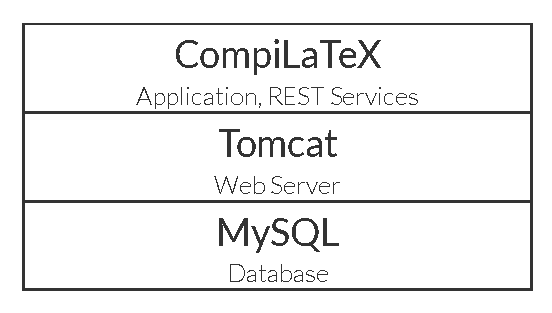
\includegraphics[width=0.5\textwidth]{images/compilatex_architecture.pdf}
	\caption{Architecture of CompiLaTeX}
\end{figure}

\pagebreak

The execution of unit tests is achieved with \name{TestNG} while integration tests make additional use of \name{RestAssured}.

For the compilation of \LaTeX files, it uses the \name{Apache Common Exec} library and requires to be run on Linux with a fully installed \name{TexLive} distribution.

\subsubsection{Model}
\label{subsubsec:compilatex-model}
There are two models for the mapping of the \LaTeX document compilation. \class{Job} is an entity that contains a collection of all document files and the name of the directory they reside. \class{JobFile} is the entity for a document file, it holds the name of the file, the parent folder, the date when it was modified last and if it is the main file, therefore to be used as target for the compilation engine.

Both entity classes have also a \name{Data Transfer Object} (\abk{DTO}{Data Transfer Object}) representation that excludes any behavior except for storage and retrieval of its own data, therefore not exposing business objects to REST services.

Operations in the persistence layer of the application are performed on DTOs exlusively, who are converted to entities before storing them in the data base. Entities are converted to DTOs vice versa when returning fetching data from the database.

\subsubsection{Services}
\label{subsubsec:compilatex-services}
The compilation of LaTeX documents is an autonomous, low-level task, involving basic file input/output operations and the execution of shell commands. Due to the fact that there are no known tools or plugins to capsulate the compilation of \LaTeX files for the Java programming language, such security critical functionality must be exposed as a service to external systems.

Hence it was implemented as a RESTful web service, providing a flexible way to compile \LaTeX \\ documents from any front-end using any technology. The distinct feature is not only its implementation, enabling the quick recompilation of marginally changed documents by updating only individual modified files or resources, but the dynamic support of \LaTeX environments.

The typical scenario for CompiLaTeX is the following: Several documents are posted to the server, then it is queried for the available compiler engines. The compilation with a given engine is requested and either the log or the \fileformat{PDF} or both can be retrieved afterwards. Before recompiling a document, the recent versions of changed files can be sent to the server and updated there. Then the document can be recompiled using the same or a different engine, requesting the log or \fileformat{PDF} afterwards.

In the following, there will be an overview given over the available REST services, ordered by resource. The presented URLs are usually prefixed with \parametertype{/rest/} but this is omitted in the following depictions for the sake of simplicity.

\headline{Latex}

The Latex resource has only a single service for the exposure of all available \LaTeX engines and is typically requested before document compilation. Since the information about the available latex compiler should be accessible at all times, they are publicly exposed.

\rest{Get Available \LaTeX Environments}
{POST}{latex/environments}
{}{APPLICATION\_JSON}
{LatexEnvironment[]}

\headline{Jobs}

The Jobs resource has multiple services for the handling of compilation jobs. Jobs can be created, updated, deleted, the compilation of a document performed. The log can be either requested as plain text or formatted with HTML elements, so can the created \fileformat{PDF} file. The log and \fileformat{PDF} can only be requested when a compilation occured beforehand, the latter even only after a success of such.

\rest{Create New Job}
{POST}{/jobs}
{}{APPLICATION\_JSON}
{JobDTO}

\rest{Compile Job}
{GET}{/jobs/\{jobId\}/compile/\{latexEnvironment\}}
{}{APPLICATION\_JSON}
{}

\rest{Get Job Log}
{GET}{/jobs/\{jobId\}/log}
{}{TEXT\_PLAIN}
{Log}

\rest{Get Job HTML Log}
{GET}{/jobs/\{jobId\}/log/html}
{}{TEXT\_PLAIN}
{String also containing HTML tags}

\rest{Get Job PDF}
{GET}{/jobs/\{jobId\}/pdf}
{}{APPLICATION\_OCTET\_STREAM}
{String}

\rest{Delete Job}
{DELETE}{/jobs/\{jobId\}}
{}{APPLICATION\_JSON}
{}

\headline{Job Files}

All services involving files need to be called with the \parameter{jobId} and \parameter{filed} as parameter, except adding a file. Both adding and updating a file consume input streams and return the resource as JSON.

To determine if a given resource resides in an outdated version on the server, the last file modification date can be requested. The response then contains the unix system time when it was last modified, therefore added or updated, on the server.

\restwithtwoparam{Add File}
{POST}{/jobs/\{jobId\}/files}
{MULTIPART\_FORM\_DATA}{}
{file}{FileInputStream}
{isMainTex}{boolean}

\restwithtwoparam{Update File}
{PUT}{/jobs/\{jobId\}/files/\{fileId\}}
{MULTIPART\_FORM\_DATA}{APPLICATION\_JSON}
{file}{FileInputStream}
{filename}{String}

\rest{Get Last File Modification Date}
{GET}{/jobs/\{jobId\}/files/\{fileId\}/lastchanged}
{}{TEXT\_PLAIN}
{JobFileDTO}

\rest{Delete File}
{DELETE}{/jobs/\{jobId\}/files/\{fileId\}}
{}{}
{no content}

\subsubsection{Implementation}
\label{subsubsec:compilatex-implementation}
The compilation of documents is organised in jobs, each having its unique directory on the server to upload files to, store logs and created PDFs. The directory name is represented by a Universally Unique Identifier (\abk{UUID}{Universally Unique Identifier}), generated upon creation of a new job and may for instance look like this: 550e8400-e29b-11d4-a716-446655440000.

When files are added or updated, input streams are read and written to the file system, in the job's directory, with the given filename. If the \parameter{jobId} URL parameter can not be mapped to a job, an error is returned in the response. Adding a file to a job also requires a parameter to indicate if it is the main \LaTeX file.

\headline{Compilation}

To compile a document, the corresponding job must contain a file being marked as main \fileformat{.tex} file. This is required to decide which file of a job is the actual target of the compilation, then achieved by using the \name{Apache Commons Exec} library which can securely and reliably execute external processes \cite{website:apache-commons-exec}.

\pagebreak

\begin{lstlisting}[language=Java, caption=Executing the Compilation of \LaTeX Files by Command Line]
/* cd to project directory */
executor.setWorkingDirectory(new File(jobDirectory));

/* build command */
CommandLine commandLine = new CommandLine(latexEnvironment.name().toLowerCase());
commandLine.addArgument("-interaction=batchmode");
Map map = new HashMap();
map.put("file", filename);
commandLine.addArgument("${file}");
commandLine.setSubstitutionMap(map);

/* execute command */
executor.execute(commandLine, resultHandler);
\end{lstlisting}

When calling the service to compile a document, a parameter is passed along, indicating which environment will be used for compilation. Prior to compilation, it is verified that this environment is actually installed on the system, returning an error in the response if it is not the case. For this, the \method{which} command is used on Linux systems.

Before compilation, the working directory is changed to the job directory. Then, the command is iteratively created, first adding the command by setting the compilation engine, then the adding parameter for the interaction mode and file name. Finally, the compilation is executed.

\headline{Log and \fileformat{PDF}}

After the compilation, both the log and \fileformat{PDF} can be requested, although the latter only after successful execution of the compilation. If so, the log or \fileformat{PDF} are read from the file system and returned. 

The process of returning the log with HTML markup is slightly more sophisticated. The log file is read into a String and searched for warnings and errors. Regular expressions will then enclose these warnings and errors with HTML markup. That way, they can later easier be styled in the front-end. And also, regular line breaks are replace by their HTML equivalent.

\headline{Available Environments}

Available \LaTeX engines for compilation are publicly exposed by REST. When requesting a list of the installed engines on the server, all values from the Enum \class{LatexEnvironment}, containing engines like \name{PDFLATEX}, \name{LUATEX}, \name{XETEX}, are fetched. Then for each is tested if it is installed on the server and added to the response. 

\pagebreak

This allows for the service to provide all \LaTeX environments dynamically, being able to add, update or remove them by installing or uninstalling their corresponding packages in the system without having to restart the server. Although this is only required when adding new engines that are not yet defined in the \class{LatexEnvironment} class. 

To avoid this slight inconvenice, it is conceivable to switch from the use of an Enum to a properties file for instance.

\subsubsection{Tests}
\label{subsubsec:compilatex-tests}

There are several unit tests in CompiLaTeX covering various aspects of the system. There are tests for the conversion between entities and DTOs, tests for the execution of the compilation by shell and tests for the persistence layer and database access.

These tests can be executed by invoking the Maven test target.

\begin{lstlisting}[caption=Invoke Unit Tests in CompiLaTex]
mvn test
\end{lstlisting}

However, this does not include the test of REST services, as they require the actual deployment of the application on a web server. The test of these services are convered by the integration tests, which can be run by invoking the following Maven target.

\begin{lstlisting}[caption=Running Integration Tests in CompiLaTex]
mvn verify
\end{lstlisting}

Integration tests simulate the actual use of a system in production mode. They assure the accurate functioning of the business logic, persistence layer, components that have already been tests in unit tests, and their flawless interaction with each other.

To deploy the application on a web server for testing purposes, two Maven plugins are used. The first, \name{failsafe} invokes the target \parameter{verify} and specifies which tests are to run.

The second controls the server by starting and shutting it down prior and posterior to the tests, specifying the port and root path. 

\pagebreak

\begin{lstlisting}[caption=Integration Tests Configuration in CompiLaTex]
<plugin>
    <groupId>org.apache.maven.plugins</groupId>
    <artifactId>maven-failsafe-plugin</artifactId>
    <version>2.17</version>
    <configuration>
        <includes>
            <include>**/*ServiceTest*</include>
        </includes>
    </configuration>
    <executions>
        <execution>
            <goals>
                <goal>integration-test</goal>
                <goal>verify</goal>
            </goals>
        </execution>
    </executions>
</plugin>

<plugin>
    <groupId>org.apache.tomcat.maven</groupId>
    <artifactId>tomcat7-maven-plugin</artifactId>
    <version>2.2</version>
    <configuration>
        <path>/</path>
    </configuration>
    <executions>
        <execution>
            <id>start-tomcat</id>
            <phase>pre-integration-test</phase>
            <goals>
                <goal>run</goal>
            </goals>
            <configuration>
                <port>9090</port>
                <fork>true</fork>
            </configuration>
        </execution>
        <execution>
            <id>stop-tomcat</id>
            <phase>post-integration-test</phase>
            <goals>
                <goal>shutdown</goal>
            </goals>
        </execution>
    </executions>
</plugin>
\end{lstlisting}

\subsection{CollaboraTeX}
\label{subsec:collaboratex}
CollaboraTeX is the web application for the collaborative editing of \LaTeX documents. It is written in Java and based on the Google App Engine platform, but runs on AppScale. That in turn is installed on OpenStack, which is utilised by the ITM Cloud Computing Lab to provide a \nameref{subsubsec:iaas}. This is illustrated in the following architecture depiction:

\begin{figure}[H]
	\centering
		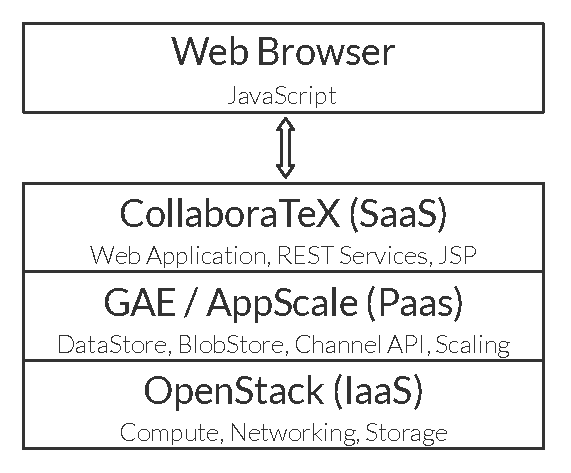
\includegraphics[width=0.5\textwidth]{images/collaboratex_architecture.pdf}
	\caption{Architecture of CollaboraTeX}
\end{figure}

CollaboraTeX makes use of lots of different Java frameworks and libraries and relies on \name{Maven} for the dependency management of them. First and foremost, the \name{AppEngine SDK} is needed to develop applications on Google App Engine. Because there are some features that are handled differently on its parallel architecture than in classic server environments, libraries for \name{DataNucleus} are also required. 

\name{DataNucleus} provides the transparent persistence of Java objects, which is here realised with JPA and EclipseLink, supporting various datastore models such as relational datastores, object-based datastores, document-based storage and more \cite{website:data-nucleus}. Before entity classes can be persisted, they must be "enhanced" by \name{DataNucleus}, which is essentially a mechanism that byte-code manipulates classes between compilation and runtime. The process itself will not be further explained, but the corresponding resources can be consulted \cite{website:data-nucleus-enhancement}.

Several of the services provided by the Google App Engine platform are used. When persisting data, they are stored in the \name{DataStore}, which has a quota of 1 megabyte and is mostly used for entities.

\pagebreak

Google describes the \name{DataStore} as:

\begin{quote}
App Engine's data repository, the High Replication Datastore (HRD), uses the Paxos algorithm to replicate data across multiple datacenters. Data is written to the Datastore in objects known as entities. Each entity has a key that uniquely identifies it. An entity can optionally designate another entity as its parent; the first entity is a child of the parent entity. The entities in the Datastore thus form a hierarchically-structured space similar to the directory structure of a file system. An entity's parent, parent's parent, and so on recursively, are its ancestors; its children, children's children, and so on, are its descendants. An entity without a parent is a root entity \cite{website:gae-datastore}.
\end{quote}

In contrast, the \name{BlobStore} is used for larger files:

\begin{quote}
The Blobstore API allows your application to serve data objects, called blobs, that are much larger than the size allowed for objects in the Datastore service. Blobs are useful for serving large files, such as video or image files, and for allowing users to upload large data files. Blobs are created by uploading a file through an HTTP request. Typically, your applications will do this by presenting a form with a file upload field to the user. When the form is submitted, the Blobstore creates a blob from the file's contents and returns an opaque reference to the blob, called a blob key, which you can later use to serve the blob. The application can serve the complete blob value in response to a user request, or it can read the value directly using a streaming file-like interface \cite{website:gae-blobstore}.
\end{quote}

\label{gae-services}
So CollaboraTeX uses the \name{DataStore} to store all entities for projects and project files, while the actual files for a \LaTeX document, also including images, the bibliography and so forth, are stored in the \name{BlobStore}.

Furthermore, a service of the Google App Engine is used that is called \name{Channel API}. It is utilised to keep persistent connections between associated clients and the application. This allows to send and receive data for document updates and synchronisation to JavaScript clients in real time \cite{website:gae-channel-api}. This technique is also known as server-push.

The search is implemented with the GAE \name{Search API} \cite{website:gae-search-api}.

\name{Jersey} is the chosen implementation of the \name{Java API for RESTful Web Services}.

For testing, \name{TestNG} and \name{RestAssured} are used, the latter for integration tests.

As \nameref{subsubsec:saas}s are commonly built as a web application that can be accessed with a simple browser, the same applies to CollaboraTeX, being most appropriate for an online \LaTeX editor. \name{Java Server Pages} are used to dynamically generate and deliver web pages based on the Hypertext Markup Language (\abk{HTML}{Hypertext Markup Language}). It integrates \name{Bootstrap} as front-end framework and makes heavy use of the library \name{jQuery} for JavaScript code \cite{website:bootstrap} \cite{website:jquery}.

\subsubsection{Model}
\label{subsubsec:collaboratex-model}
There are three models in CollaboraTeX, two to reflect \LaTeX documents and one class for the user management,  authentification and sharing.

\class{Project} is the entity that contains the name of the project and a collection of all document files. A document file again is modelled by the entity \class{ProjectFile}, it holds the name of the file, the content type, the size, the date when it was modified last and if it is the main file, to indicate it as the target for the compilation engine. Besides, the class is storing the \parameter{BlobKey} that uniquely indentifies the stored file in the BlobStore. As previously mentioned, this is necessary since the Google App Engine platform is not based on a file system. Data are stored either in the DataStore, which is mostly for persisting entities, or the BlobStore, which is used for larger files.

The \class{User} entity does contain the username, which is used to map it to LDAP services, and collections for owned projects, meaning write and read access, and accessible projects, signifying read access only.
 
All three entity classes have \name{Data Transfer Object} (DTO) representations that exclude any behavior except for storage and retrieval of its own data, to prevent the exposure of business objects via REST services.

Operations in the persistence layer are performed on \name{Data Access Objects} (DAO). They make use of the DTOs, converting them to entities before storing them in the data base. In reverse, entities are converted to DTOs before returning fetched data from the database.

\subsubsection{Services}
\label{subsubsec:collaboratex-services}
The front-end communicates with the CollaboraTeX back-end by calling its REST services, thus any actions by the user on the web page will trigger their counterparts in the back-end and change the state of the system.

A typical scenario would be this: A user logs in to the website and decides to upload an existing \LaTeX document. The files are posted to the server and a new project created, that will be displayed on the web page. When opening a \LaTeX file, a REST service is called to get the file content and display it in the editor. On changes in the document, the client will again call a service to submit them and the back-end persists the updated document state, also sending the changes to all associated clients that have the same document \LaTeX file opened. Upon compilation, everything is sent to the CompiLaTeX server and on finish, the log is requested to be displayed to the user.

The following will give an overview over the available REST services of CollaboraTeX, ordered by resource. The presented URLs are usually prefixed with \parametertype{/rest/} but this is omitted in the following depictions for the sake of simplicity.

\headline{Projects}

This resource provides multiple services for the handling of projects. They can be newly created or imported with existing files, both do not require any URL or form parameter. For the import, the files will be read from the request itself.

Projects can be renamed which requires a parameter \parameter{value} for the new name, deleted or download, all need a valid \parameter{projectId}. In the latter case, the project will be downloaded as a zipped file.

\rest{Create New Project}
{POST}{/projects}
{}{APPLICATION\_JSON}
{ProjectDTO}

\rest{Import \LaTeX Files}
{POST}{/projects/import}
{MULTIPART\_FORM\_DATA}{}
{ProjectDTO}

\rest{Download Project as ZIP File}
{GET}{/projects/\{projectId\}/download}
{}{}
{Application/ZIP}

\restwithparam{Rename Project}
{POST}{/projects/\{projectId\}/rename}
{}{APPLICATION\_JSON}
{value}{String}
{ProjectDTO}

\rest{Delete Project}
{DELETE}{/projects/\{projectId\}}
{}{}
{no content}

\headline{Project Files}

All services involving files in projects need to be called with the \parameter{projectId} and \parameter{fileId} as parameter, except getting a file upload URL, creating a new file or importing files.

There are some services being specifically for the handling of plain text files, like getting, patching and updating the file content. The difference between the two last-mentioned is that while the first changes a document by applying a patch to it, the last replaces the whole content of a text-based file. These services are needed to realise collaborative editing.

Moreover, there are services to update a file with a more recent version, renaming it, setting it as main tex file (albeit the application should be able to do an automatic detection most of the times), getting a file's meta data or deleting it.

\rest{Get File Upload URL}
{GET}{/projects/\{projectId\}/uploadurl}
{}{TEXT\_PLAIN}
{URL}

\rest{Create New File}
{POST}{/projects/\{projectId\}/files}
{MULTIPART\_FORM\_DATA}{}
{ProjectFileDTO}

\rest{Import Files}
{POST}{/projects/\{projectId\}/files/import}
{MULTIPART\_FORM\_DATA}{}
{ProjectDTO}

\rest{Get File Meta Data}
{GET}{/projects/\{projectId\}/files/\{fileId\}/meta}
{}{APPLICATION\_JSON}
{ProjectFileDTO}

\rest{Get File Content}
{GET}{/projects/\{projectId\}/files/\{fileId\}}
{}{FILE CONTENT TYPE}
{File}

\rest{Set As Main Tex File}
{POST}{/projects/\{projectId\}/files/\{fileId\}/setmaintex}
{}{APPLICATION\_JSON}
{ProjectFileDTO}

\restwithparam{Rename File}
{POST}{/projects/\{projectId\}/files/\{fileId\}/rename}
{}{APPLICATION\_JSON}
{value}{String}
{ProjectFileDTO}

\restwithparam{Patch File Content}
{POST}{/projects/\{projectId\}/files/\{fileId\}/patch}
{}{APPLICATION\_JSON}
{patch}{String}
{ProjectFileDTO}

\restwithparam{Update File Content}
{POST}{/projects/\{projectId\}/files/\{fileId\}/content}
{}{APPLICATION\_JSON}
{content}{String}
{ProjectFileDTO}    

\rest{Update File}
{PUT}{/projects/\{projectId\}/files/\{fileId\}}
{MULTIPART\_FORM\_DATA}{APPLICATION\_JSON}
{ProjectFileDTO}

\rest{Delete File}
{DELETE}{/projects/\{projectId\}/files/\{fileId\}}
{}{}
{no content}

\headline{Session}

There are session services, that are required for the synchronisation of documents in clients - and therefore enable collaborative editing in the first place.

Before a persistent connection to the client can be initiated via Channel API, it must acquire a so-called token from the server that uniquely identifies it.

To synchronise changes only with clients that have opened the same file, there are services to register and unregister for a document.

\rest{Get Channel API Token}
{GET}{/session/channel/token}
{}{TEXT\_PLAIN}
{ProjectFileDTO}

\rest{Register for an Open Document}
{POST}{/session/document/\{fileId\}/register}
{}{TEXT\_PLAIN}
{ProjectFileDTO}

\rest{Unregister for an Opened Document}
{POST}{/session/document/\{fileId\}/unregister}
{}{TEXT\_PLAIN}
{ProjectFileDTO}

\headline{Search}

The search is provided by a single service that takes a \parameter{query} as parameter and returns all found results - which are project files that matched the search criteria - as a list in JSON. 

\restwithparam{Search All Documents With Query}
{POST}{/search}
{}{APPLICATION\_JSON}
{query}{String}
{List<ProjectFileDTO>}

\subsubsection{Implementation}
\label{subsubsec:collaboratex-implementation}
Before descending into the depths of the system's implementation, the following list of features should give an idea about CollaboraTeX' functionalities:

\begin{itemize}
	\item{Creation, deletion, renaming of projects and files}
	\item{Import of existing documents and download of projects as ZIP file}
	\item{Automatic detection of \parameter{begin\{document\}} in \LaTeX files and setting them as main file}
	\item{Editor with syntax highlighting for \LaTeX}
	\item{Synchronisation of document changes for attached collaboration clients}
	\item{Immediate background persisting of document changes}
	\item{Undo and redo for local changes}
	\item{Extensive menus with most widely used \LaTeX commands}
	\item{Context menus for projects and files in the sidebar}
	\item{Keyboard shortcuts}
	\item{Inline editing of project and file names}
	\item{Search by file attributes}
	\item{Auto-completion (not only for \LaTeX commands)}
	\item{Compilation of \LaTeX files}
	\item{Viewable compilation log}
	\item{View generated \fileformat{PDF} in browser}
\end{itemize}

Hereafter, the most significant functions and their implementation details will be explained, which are \name{Import}, \name{Context Menus}, \name{Editor View}, \name{Collaboration}, \name{Compilation}, \name{Log}, \name{PDF Viewer} and \name{Search}.

%\begin{figure}[H]
%	\centering
%		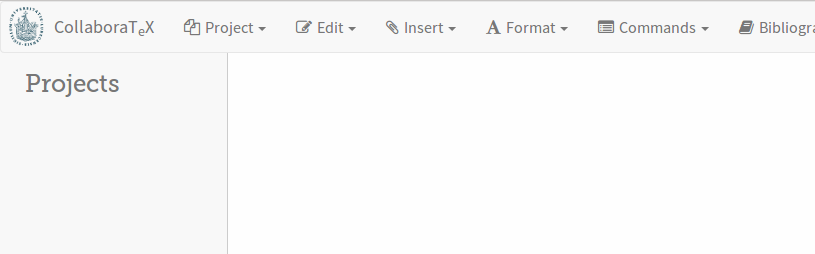
\includegraphics[width=0.8\textwidth]{images/screenshot-empty-main.png}
%	\caption{}
%\end{figure}

\headline{Import}

For the import of \LaTeX files, the front-end provides the user with a form to upload files. Files may either be selected by the filechooser or added by drag'n'drop. Files from subdirectories can be imported as well, although folders are not supported in CollaboraTeX projects because of the architecture of Google App Engine and its Blobstore (compare page \pageref{subsec:collaboratex}).

When importing a project, the project name is a required field, otherwise the form cannot be submitted. The statement of individuals that should have access to the project is an optional field. It supports autocompletion for the usernames but only as proof of concept. No user management was implemented in CollaboraTeX yet. The ultimate aim should be to aggregate the data for this by integrating the LDAP protocol.

\begin{figure}[H]
	\centering
		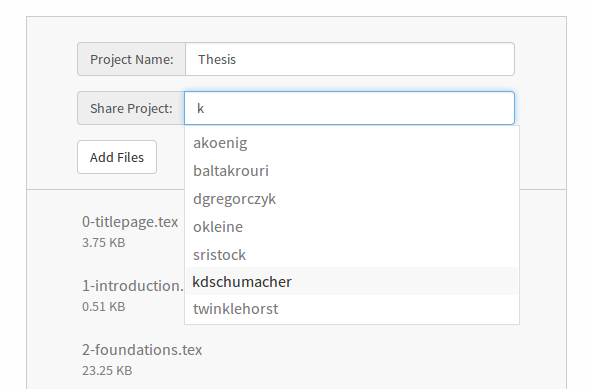
\includegraphics[width=0.66\textwidth]{images/screenshot-import-project.png}
	\caption{CollaboraTeX form to import \LaTeX documents}
\end{figure}

Upon the submit of the form, a new project is created with the given name and the files are gathered from the request. Each file is persisted in the BlobStore, added to the search index and then attached to the project, which is finally persisted itself in the DataStore.

\newpage

\headline{Context Menus}

To provide an easy and accessible way for users to control all project- and file-related actions, there are context menus for the sidebar. They  open themselves when clicking the right mouse button, are context sensible and come in three variations.

Invoking it on an empty space in the project sidebar, where projects and menus are displayed, opens a content menu that has the commands to either create a new project or import one. 

A menu with commands to share, rename, download, delete a project is openend when invoking it on a project. Additionally there are commands to create a new file or import an existing one. This is shown in the graphic below.

\begin{figure}[H]
	\centering
		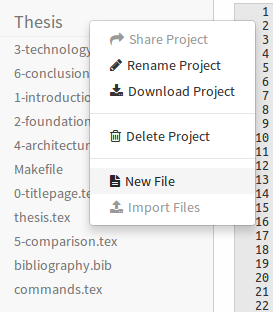
\includegraphics[width=0.35\textwidth]{images/screenshot-project-context-menu.png}
	\caption{An exemplary context menu for a project in CollaboraTeX}
\end{figure}

And then there is the context menu for files, it has options to rename a file, set it as main \TeX file or delete it.

The technical implementation for this is the following: Each item of the context menu has a unique identifier, for example:

\begin{lstlisting}[language=HTML, caption=Exemplary HTML Code for a Context Menu Item]
<li>
	<a id="newproject" class="contextmenu" tabindex="-1" href="#">
		<i class="fa fa-folder"></i> New Project
	</a>
</li>
\end{lstlisting}

For this identifier, a click handler is set in JavaScript, which performs the respective action. This handler will then execute its JavaScript code to react to the click and would typically involve a call to a REST service. \\

\begin{lstlisting}[language=JavaScript, caption=Exemplary Click Handler in JavaScript for a Context Menu Item]
$('a#newproject.menu, a#newproject.contextmenu').on('click', function() {
	$.post("/rest/projects", function(data) {
        /* create project entry in sidebar */
        createEmptyProjectList(data.id, data.name);

        /* make project name editable */
        $("a[data-pk='" + data.id + "']").editable();
        
        /* set context menu or it wouldn't be instantly available */
        setProjectContextMenu();
    });
});
\end{lstlisting}

\headline{Editor View}

The key feature of the editor view is the integrated \name{ACE Editor}. It is highlighting the syntax of a \LaTeX file, has an internal stack for redo and undo operations and features code-completion, keyboard shortcuts and much more. On the top left of the editor is a tab showing the name of the file and a button to close the editor. Also above the editor but on the right is a toolbar for the compilation. First, all available compilation engines are displayed (here PdfLaTeX) in a drop down menu, then there are buttons for the compilation, viewing the \fileformat{PDF} and the log.

\begin{figure}[H]
	\centering
		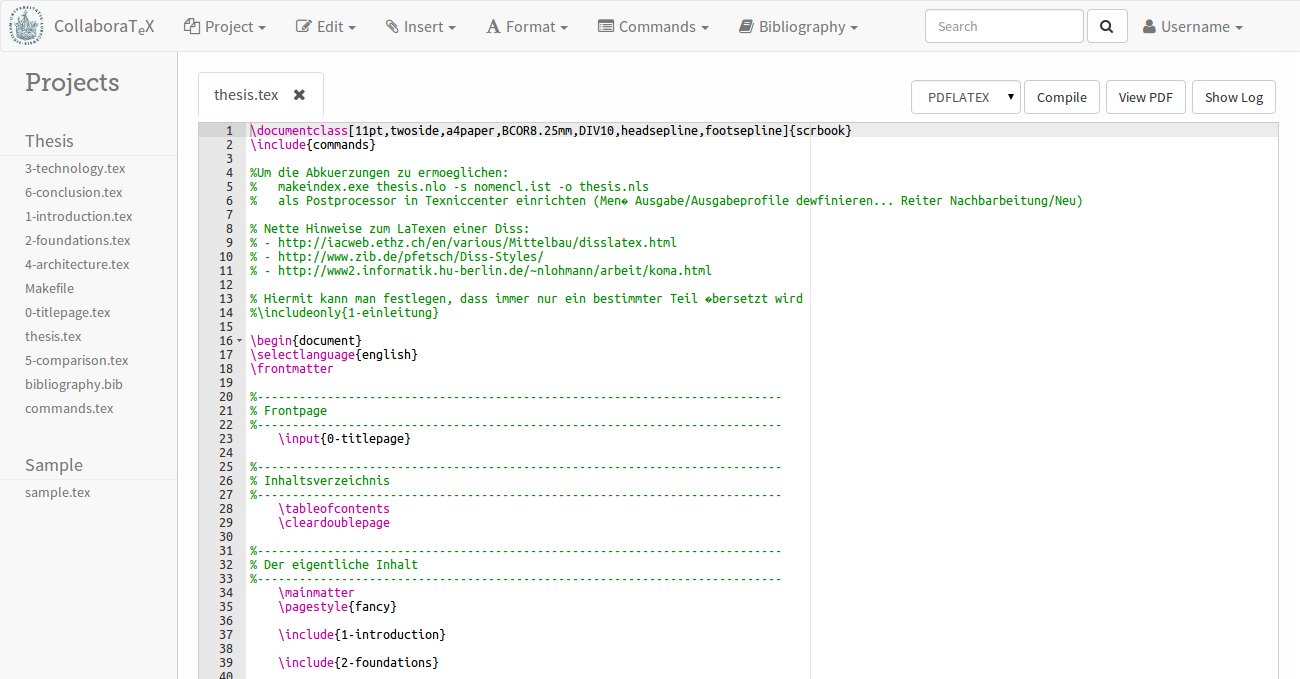
\includegraphics[width=\textwidth]{images/screenshot-editor.png}
	\caption{The editor view in CollaboraTeX}
\end{figure}

\pagebreak

A file is shown in the editor when it was clicked in the sidebar. The click handler is first checking if the main page for editor is opened and then if the chosen file is actually text-based and not in a format that could not be opened by the editor, for instance images. A service call is made to register the client for the openend document. The content of the file is then requested by calling the REST service and the response set as the editors content, displaying the file.

If the close button for the tab is clicked, a service call is made to unregister the client for the document and the editor is closed.

Undo and redo operations work only for local changes.

\headline{Collaboration}

To describe how the collaborative editing is implemented in CollaboraTeX, it will follow the typical use case of two users working together on a document at the same time. It is assumed that both users have opened the same document already and are therefore registered for it in the back-end.

To detect changes in a document, a library is used that is called jQuery Typing, developed by Maciej Konieczny \cite{website:jquery-typing}. It is rather old and straightforward, but serves its purpose. That is to detect the begin and end of a user typing. It is used here to calculate the changes and send them to the server if a user pauses his input.

\begin{lstlisting}[language=JavaScript, caption=Typing Listener for the Editor]
$('#editor > textarea').typing({
    start: function() {
        originalText = ace.edit('editor').getSession().getValue();
    },
    stop: function() {
        var patch = getPatch(originalText);
        sendChangesToServer(patch);
    },
    delay: 400
});
\end{lstlisting}

So when a user starts to type, the content of the editor is saved in a global variable \parameter{originalText}. If the typing is then paused for at least 400 milliseconds, the user is thought to have ended his input. First, a patch of the document changes based on the stored original content is calculated and then sent to the server.

For the all text-related operations that are the base for \nameref{subsubsec:operational-transform}, such as creating diffs and patches, the \name{Google Diff Match Patch} library is used in JavaScript.

\pagebreak

\begin{lstlisting}[language=JavaScript, caption=Creation of a Diff and subsequently a Patch for the Document's Changes]
function getPatch(originalText){
	var dmp = new diff_match_patch();

	/* calculate diff from original and current text */
	var currentText = ace.edit('editor').getSession().getValue();
	var diff = dmp.diff_main(originalText, currentText, true);

	/* make patch from diff and original and current text */
	var patch_list = dmp.patch_make(originalText, currentText, diff);
	var patch = dmp.patch_toText(patch_list);

	return patch;
}
\end{lstlisting}

The patch is then passed to a function not cited here, that gathers the \name{projectId} and \name{fileId}. Finally the patch is posted to the REST resource.

\begin{lstlisting}[language=JavaScript, caption=Posting the Patch to the REST Service]
function patchFileContent(projectId, fileId, patch) {
    $.post('/rest/projects/' + projectId + '/files/' + fileId + '/patch', {patch: patch}, function(data) {
        /* not much to do on success */
    });
}
\end{lstlisting}

After the server receives the patch, it first fetches the \class{Project} object with the given \parameter{projectId} and then the \class{ProjectFile} object for the given \parameter{fileId}. On the server, the same library is used as in the client, \name{Google Diff Match Patch}, which is important to achieve not only the synchronisation between clients but also across all clients and the server.

To possess the most recent version of the document on the server then amounts to the easy task of applying the patch on the current state of the document as the server knows it.

\begin{lstlisting}[language=Java, caption=Applying the Patch for a Document on the CollaboraTeX Server]
private String createPatchedContent(String patch, String content) throws IllegalArgumentException {
    /* create diff match patch instance */
    diff_match_patch dmp = new diff_match_patch();
    
    /* create single patches from text patch and apply to file content */
    List<Patch> patches = dmp.patch_fromText(patch);
    Object[] results = dmp.patch_apply((LinkedList<Patch>) patches, content);
    
    /* first array entry contains patched text  */
    return (String) results[0];
}
\end{lstlisting}

As there is no possibility to update files that are stored in the BlobStore, the old version of the file is deleted from it first, then the new patched version is written to the BlobStore and all references in the \class{ProjectFile} object are updated, such as the \parameter{blobKey} and \parameter{lastChanged} date. This ensures that all changes to the document are persisted immediately.

The search index however is able to update existing data, so the new file is simply put to it and the index updated accordingly.

The last and maybe most important step is that the changes are broadcasted to all clients that are currently editing the same document. This is achieved by using the Google App Engine Channel API, thus implementing a server push where the web server leaves a connection open to send out data on events to the client immediately \cite{burke2013restful}. 

These connections are created on the client-side when a user accesses the website, their lifetime is two hours.

\begin{lstlisting}[language=Java, caption=Broadcast Changes to All Associated Clients Having the Same Document Opened]
private void pushPatchToAllAssociatedClients(Long fileId, String patch, String originSessionId) {
        
        /* get map of all opened documents */
        Map<String, Long> openedDocuments = SessionManager.getOpenedDocuments();
        for (Entry<String, Long> entry : openedDocuments.entrySet()) {
            
            /* get session and document id */
            String sessionId = entry.getKey();
            Long documentId = entry.getValue();
            
            /* send patch to client if it has opened the same file and was NOT the one who made the changes */
            if (documentId.equals(fileId) && !sessionId.equals(originSessionId)){
                channelService.sendMessage(new ChannelMessage(sessionId, patch));
            }
        }
    }
\end{lstlisting}

The Channel API declares standard functions in JavaScript that are executed on the client-side when receiving any data from the server. Those are \method{onOpen}, \method{onMessage}, \method{onError} and \method{onClose}. 

Here the \method{onMessage} function is used to receive and process the message from the server containing the patch.

\pagebreak

\begin{lstlisting}[language=JavaScript, caption=Apply the Broadcasted Patch From the Server on the Client]
function onMessage(patch) {
    if ($('#editor')) {
        var dmp = new diff_match_patch();

        /* apply patch to current editor content */
        var currentText = ace.edit('editor').getSession().getValue();
        var patches = dmp.patch_fromText(patch.data);
        var results = dmp.patch_apply(patches, currentText);

        /* set patched content as new content */
        ace.edit('editor').getSession().setValue(results[0]);
    }
}
\end{lstlisting}

\label{simpler-ot-reason}

When comparing this approach to the pure theory of \nameref{subsubsec:operational-transform} it strikes the eye that this implementation is a simpler version of it. It does not take into account that the transit time of messages between clients and server, while two or more users edit the document in real-time, can lead to conflicts, as updates can be outdated by the time they will either reach the server or the client.

This is due to two major reasons: On the one hand, it is assumed that delay of messages, high transit times or even loss of connection are ruled out in the target environment, the ITM Cloud Computing Lab. 

On the other hand, the lack of \nameref{subsubsec:operational-transform} libraries that can be used with a Java back-end makes it neccessary to write the logic behind it from scratch. Given the time and scope of this work, this proved to be unfeasible.

\headline{Compilation}

The compilation is triggered from the toolbar above the editor. When opening the editor, a request to a CompiLaTeX REST service is made to get the available compilation engines and display them as a drop down menu (compare page \pageref{subsubsec:compilatex-services}). 

The toolbar also provides buttons for the compilation, to view the \fileformat{PDF} and the log. In case of non-reachability of the CompiLaTeX server, a hint that compilation is currently not possible is shown instead of the toolbar.

The communication and interaction among both servers can be seen in the graphic below. To create no interdependencies between them, all service calls are made by JavaScript in the client. However, they could directly communicate with each other on the application layer by consuming their REST services.

\begin{figure}[H]
	\centering
		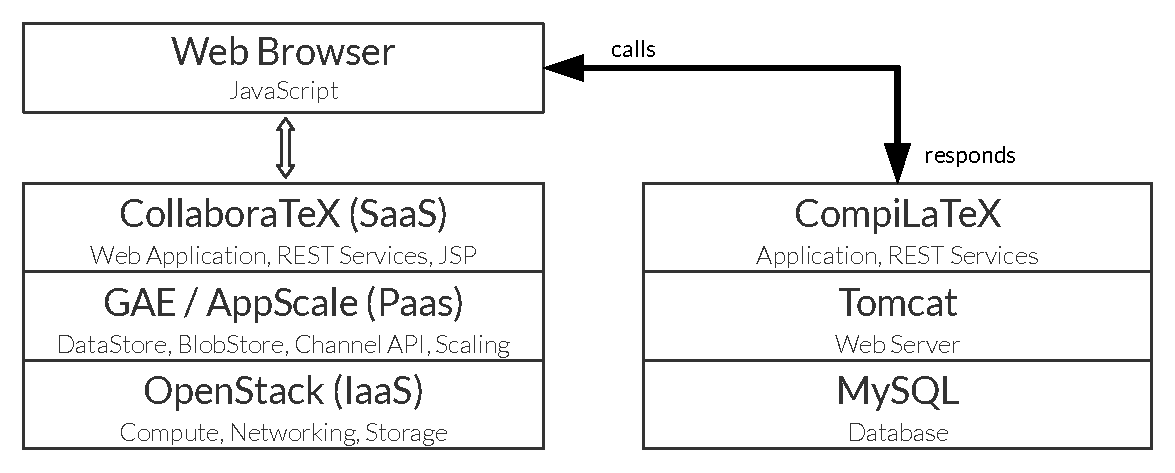
\includegraphics[width=\textwidth]{images/cotex_architecture.pdf}
	\caption{Interaction between CollaboraTeX and CompiLaTeX}
\end{figure}

When triggering the compilation, the following things happen throughout the process. Initially, a service call is made to CompiLaTeX to create a new job. Then all files are gathered and posted by the function \method{addFile} to the recently created CompiLaTeX compilation job. 

When all files were transfered to the CompiLaTeX server, the compilation can be invoked by yet another service call with the parameters \parameter{jobId} and the chosen \parameter{latexEnvironment}. Upon completion, the log for the job is requested and appended to a div the CollaboraTeX webpage, as well as the compilation time is displayed right next to the toolbar.

\begin{lstlisting}[language=JavaScript, caption=Click Listener for the Compilation Button in CollaboraTeX]
/* get latex environment for compilation from select */
var latexEnvironment = $('#latexenvironment option:selected').text();
/* create job by posting to CompiLaTeX service */
var job = createNewJob();

/* get project files */
var projectId = getProjectIdFromTab();
var fileIDs = getProjectFileIDsFromSidebar(projectId);
for (var i = 0; i < fileIDs.length; i++) {
	/* add them to CompiLaTeX Job by posting to its service */
    var fileId = fileIDs[i];
    var fileMetaData = getFileMetaData(projectId, fileId);
    var content = getFileContent(projectId, fileId);
    var createdFile = addFile(job.id, content, fileMetaData.name, fileMetaData.mainTex);
}

/* compile and append log to div#log*/
compileJob(job.id, latexEnvironment);
appendLogToPage(getHtmlJobLog(job.id));
\end{lstlisting}

How the compilation is achieved in CompiLaTeX is described in \nameref{subsubsec:compilatex-implementation} on page \pageref{subsubsec:compilatex-implementation}.

\headline{Log}

As previously mentioned, the log is appended to a collapsible div after compilation. It can be shown or hidden by clicking the corresponding button in the compilation toolbar above the editor.

The log is presented in a webpage-optimised way, meaning that errors and warnings that occured during the compilation are coloured in red, respectively yellow, throughout the log to let the user spot them more easily. Their number of occurrences is also summarised in the headline.

\begin{figure}[H]
	\centering
		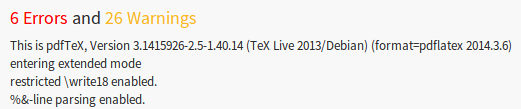
\includegraphics[width=0.66\textwidth]{images/screenshot-compile-log-warning.png}
	\caption{Log for erroneous compilation with coloured errors and warnings}
\end{figure}

If the compilation went well, so no errors occured and the output (\fileformat{PDF}) could be successfully created, the most important information are summarised in the headlines of the log, showing the filename, number of pages and filesize.

\begin{figure}[H]
	\centering
		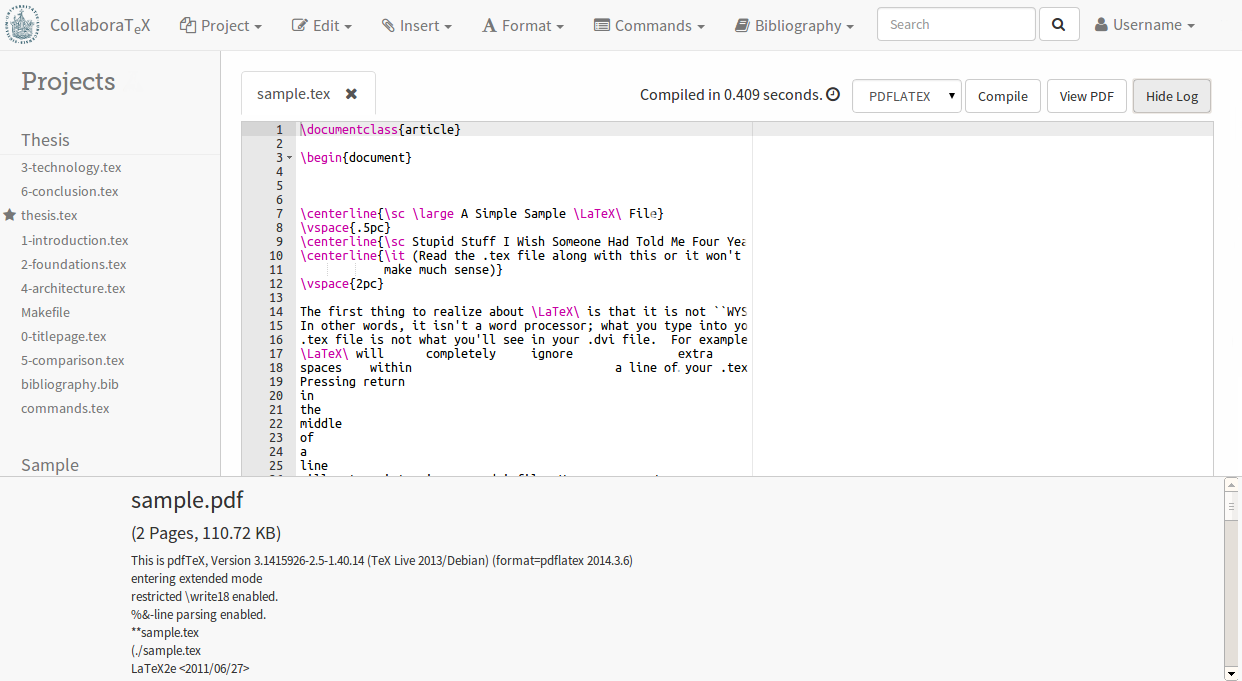
\includegraphics[width=\textwidth]{images/screenshot-compile-log-success.png}
	\caption{Log for successful compilation with summarised document information}
\end{figure}

\pagebreak

\headline{PDF Viewer}
\label{pdf-viewer}

To allow users to quickly see the generated document, \name{PDF.js} is embedded into CollaboraTeX, a \fileformat{PDF} viewer written in JavaScript which describes itself as a "web standards-based platform for parsing and rendering PDFs" \cite{website:pdf-js}.

Integrating it has multiple advantages. To begin with, it allows the operating system independent view of \fileformat{PDF} files, as it is uncertain which operating system a user of the online \LaTeX editor might use and if it has an installed \fileformat{PDF} application. Secondly, it is easier for the user to instantaneously display the file in the browser than having him to download and open it with a native application.

PDF.js is localised for various languages and offers rich and extensive features to view \fileformat{PDF}s. The page previews can be seen in a hideable sidebar, there is a search function, jump to page, zooming, fullscreen view, printing and bookmark support and the file can directly be saved.

How the \fileformat{PDF} view looks like can be seen from the following sample document:

\begin{figure}[H]
	\centering
		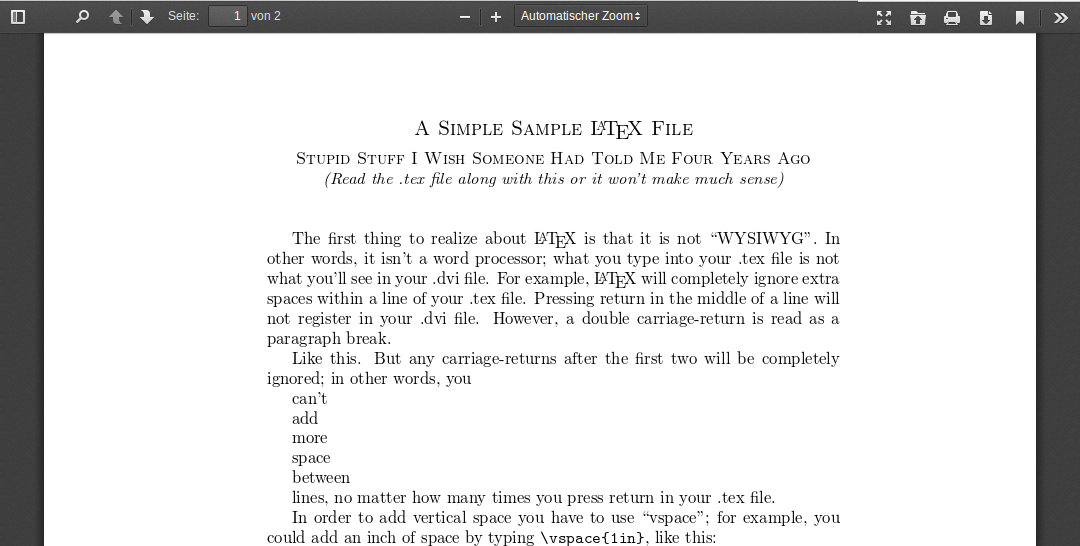
\includegraphics[width=\textwidth]{images/screenshot-pdf-viewer.png}
	\caption{Embedded \fileformat{PDF} viewer in CollaboraTeX}
\end{figure}

\headline{Search}

The search is realised with the Google App Engine \name{Search API} \cite{website:gae-search-api}. It provides a model for the indexing of documents that contain structured data and persists them in a store that is optimised for search operations. While the number of documents in such an index is unlimited, the search cannot return more than 10,000 matches. Nevertheless, this is more than sufficient for the needs of this \LaTeX editor.

Entries are represented in the search index as documents. To add files to the search index, a document must be build. Such a document can have fields with different primitive values like text, a number, a date, a locale. The fields are here populated with the file's attributes, as the code excerpt shows below. After creation, the document can be added to the search index.

\begin{lstlisting}[language=Java, caption=Building a Document Entry for the Search Index]
Document newDoc = Document.newBuilder().setId(String.valueOf(fileDTO.getId()))
    .addField(fb.setName("key").setText(fileDTO.getKey().getId()))
    .addField(fb.setName("blobKey").setText(fileDTO.getBlobKey()))
    .addField(fb.setName("name").setText(fileDTO.getName()))
    .addField(fb.setName("contentType").setText(fileDTO.getContentType()))
    .addField(fb.setName("size").setText(fileDTO.getSize()))
    .addField(fb.setName("lastChanged").setText(fileDTO.getLastChanged()))
    .addField(fb.setName("mainTex").setText(fileDTO.isMainTex())).build();

IndexSpec indexSpec = IndexSpec.newBuilder().setName("IndexName").build();
Index index = SearchServiceFactory.getSearchService().getIndex(indexSpec);
index.put(document);
\end{lstlisting}

When a user now uses the search functionality in the front-end, the query is posted by Java-Script to the according CollaboraTeX REST service and executed on the search index. To retrieve results from the search index, a simple method call is sufficient.

The results are returned as a list. For each document in it, the fields are re-mapped and a \class{ProjectFile} object is constructed. This is then added to a list of found files, finally returning it as JSON response to the client.

\begin{lstlisting}[language=Java, caption=Retrieving Results from the Search Index for a Query]
Results<ScoredDocument> results = SearchIndexManager.INSTANCE.retrieveDocuments(query.trim());
/* get attributes for each found document */
for (ScoredDocument document : results) {
    Key key = KeyFactory.createKey(document.getField("key").getText());
    BlobKey blobKey = new BlobKey(document.getField("blobKey").getText());
    String name = document.getField("name").getText();
    String contentType = document.getField("contentType").getText();
    long size = document.getField("size").getText();
    long lastChanged = document.getField("lastChanged").getText();
    boolean mainTex = document.getField("mainTex").getText();

    /* create file dto and add to found list */
    ProjectFileDTO fileDTO = new ProjectFileDTO(blobKey, name, contentType, size, lastChanged, mainTex);
    fileDTO.setKey(key);
    foundFiles.add(fileDTO);
}
return Response.ok().entity(foundFiles).build();
\end{lstlisting}

Upon reception of the results in the client, all found matches will be displayed in a table to the user. The number of matches and the performed query are both stated in the headline. The list itself is containing the different file attributes name, content type, filesize, date of last modification and if the file is set as main \TeX file.

\begin{figure}[H]
	\centering
		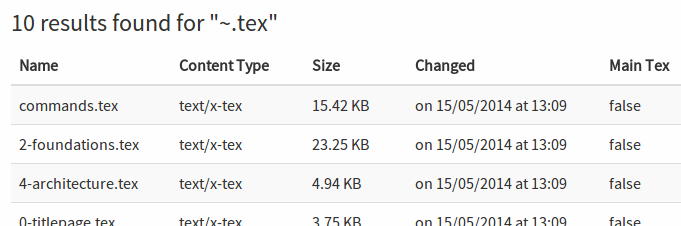
\includegraphics[width=0.8\textwidth]{images/screenshot-search.png}
	\caption{Search results are displayed in a table in CollaboraTeX}
\end{figure}

\label{reason-no-full-text-support}
As can be seen, the search does not yet provide full-text support. Although it would require minor effort to implement it, the way in which the search index is implemented on Google App Engine would pose a problem to the task of both providing the possibility to search a file's contents and its attributes. This is, that such an additional field for the content of a document has to be a Null value for non-text content types.

The full-text search is not considered to be of such importance that the examination of this problem was a priority and remained lastly unimplemented.

\subsubsection{Tests}
\label{subsubsec:collaboratex-tests}

Unit testing covers methods of a class and is used to assure their correct functioning. They are here utilised to test the conversion between entities and DTOs and the  access to the persistance layer by using Data Access Objects. These unit tests can be executed by invoking the Maven test target.

\begin{lstlisting}[caption=Invoke Unit Tests in CollaboraTeX]
mvn test
\end{lstlisting}

As the unit tests cover only basic and simple functionalities, more in-depth application tests are needed to be performed in a different way. The test of REST services requires the actual deployment of the application on a web server and are covered by the integration tests, which can be run by invoking the following Maven target.

\begin{lstlisting}[caption=Running Integration Tests in CollaboraTeX]
mvn verify
\end{lstlisting}

The integration tests are used to simulate the behaviour of the application in production mode. When using them, not only the flawless functioning of business logic, persistence layer and components that have already been unit-tested is ensured, also their interaction with one another is. 

To deploy the application for testing purposes on a Google App Engine development server, two Maven plugins need to be configured. The first, \name{failsafe} invokes the target \parameter{verify} and specifies which tests are to run. The second plugin has the task to control the start and shutdown of the server. It does so prior and afterwards to the tests.

\begin{lstlisting}[caption=Integration Tests Configuration in CollaboraTeX]
<plugin>
    <groupId>org.apache.maven.plugins</groupId>
    <artifactId>maven-failsafe-plugin</artifactId>  
    <version>2.17</version>  
    <configuration>  
        <includes>  
            <include>**/*ServiceTests.java</include>
        </includes>  
    </configuration>  
    <executions>
        <execution>  
            <phase>integration-test</phase>
            <goals>  
                <goal>integration-test</goal>  
                <goal>verify</goal>
            </goals>  
        </execution>  
    </executions>  
</plugin>

<plugin>
    <groupId>com.google.appengine</groupId>
    <artifactId>appengine-maven-plugin</artifactId>
    <version>${appengine.version}</version>
    <executions>
        <execution>
            <phase>pre-integration-test</phase>
            <goals>
                <goal>devserver_start</goal>
            </goals>
        </execution>
        <execution>
            <phase>post-integration-test</phase>
            <goals>
                <goal>devserver_stop</goal>
            </goals>
        </execution>
    </executions>
</plugin>
\end{lstlisting}

\pagebreak


